\documentclass{beamer}
\usepackage{tabularx}
\usepackage{tikz}
\usetikzlibrary{shapes.geometric, arrows}
\tikzstyle{startstop} = [rectangle, rounded corners, minimum width=3cm, minimum height=1cm,text centered, draw=black, fill=red!30]
\tikzstyle{io} = [trapezium, trapezium left angle=70, trapezium right angle=110, minimum width=3cm, minimum height=1cm, text centered, draw=black, fill=blue!30]
\tikzstyle{process} = [rectangle, minimum width=3cm, minimum height=1cm, text centered, draw=black, fill=orange!30]
\tikzstyle{decision} = [diamond, minimum width=3cm, minimum height=1cm, text centered, draw=black, fill=green!30]
\tikzstyle{arrow} = [thick,->,>=stealth]

\title{\LaTeX \ for Theses}
\subtitle{An Introductory Course}
\author{Dr Thomas Bishop \and Dr Gerard Capes}
\institute{University of Manchester}
\date{17\textsuperscript{th} November, 2016}
\logo{
\includegraphics[width=2cm]{UniOfManchesterLogo.pdf}}

\begin{document}

\begin{frame}
\titlepage
\end{frame}

\section{Introduction}

\begin{frame}
\frametitle{Staff}
\begin{itemize}
	\item Tom Bishop
	\item Gerard Capes
\end{itemize}
\end{frame}

\begin{frame}
\frametitle{Course Structure}
\tableofcontents
\end{frame}

\begin{frame}
\frametitle{What We \textbf{Won't} Be Covering}
\begin{itemize}
	\item How to use \LaTeX \ to typeset other documents (papers, reports, slides, \textit{etc}.),
	\item How to install \LaTeX \ on a Windows/Mac/Unix system,
	\item Every possible option, setting, package or trick,
	\item Image editing or drafting diagrams.
\end{itemize}
\end{frame}

\section{What Is \LaTeX?}

\begin{frame}
\frametitle{What Is \LaTeX?}
\begin{itemize}
	\item Software for typesetting.
	\item Totally free and available on many platforms.
	\item Popular in publishing technical and/or large documents.
	\item \textbf{A markup language (content and form are separated).}
\end{itemize}
\end{frame}

\begin{frame}
\frametitle{Is it For Me?}
\begin{columns}
\column{0.5\textwidth}
\begin{itemize}
	\item Produces beautiful, professional documents.
	\item There is almost certainly an elegant solution to your typesetting problem.
	\item You can logically work out how to solve an error.
\end{itemize}
\column{0.5\textwidth}
\begin{itemize}
	\item What you see isn’t what you get as you write and edit.
	\item You might have to research how to solve the problem.
	\item You will need to learn how to work with markup language.
\end{itemize}
\end{columns}

\end{frame}

\section{How \LaTeX Works}

\begin{frame} \frametitle{The Compiler}
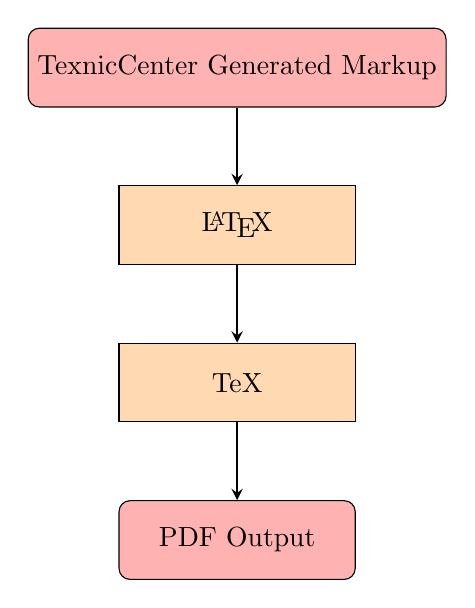
\begin{tikzpicture}[node distance=2cm]
\node (start) [startstop] 							{TexnicCenter Generated Markup};
\node (pro1)  [process, below of=start] {\LaTeX};			%both this box and the TeX box below it need to be in a larger box marked MiKTeX
\node (pro2)  [process, below of=pro1] 	{TeX};
\node (stop)  [startstop, below of=pro2] {PDF Output};
\draw [arrow] (start) -- (pro1);
\draw [arrow] (pro1) -- (pro2);
\draw [arrow] (pro2) -- (stop);	
\end{tikzpicture}
\end{frame}

\section{The University Thesis Document}

\begin{frame} \frametitle{The University Thesis Document Files}
\begin{block}{Style Sheet}
Tells \LaTeX \ how to compose the document.
\end{block}
\begin{block}{Thesis Itself}
The ``backbone'' of the document to which you add chapters.
\end{block}
\end{frame}

\end{document}